% Class
\documentclass[11pt,a4paper]{article}

% Codage
\usepackage[utf8]{inputenc}
\usepackage[T1]{fontenc}
\usepackage{siunitx}
\usepackage{indentfirst}

% Langue
\usepackage[english]{babel}

% Supplément
\usepackage{amsmath,amsfonts,amssymb}
\usepackage{verbatim} % pour faire des commentaires avec \begin{comment}...
\usepackage{float} % pour positioner un image exacetement où on veut
\usepackage
  [separate-uncertainty = true,
  multi-part-units = repeat]
  {siunitx} % Exemple \SI{0}{\kg \cdot \m^{-3}}

% Images
\usepackage[pdftex]{graphicx}
\usepackage{graphics}
\usepackage{subcaption} % pour positioner des figures côte à côte
\usepackage{wrapfig}

% pour l'inclusion de liens dans le document 
\usepackage[colorlinks,bookmarks=false,linkcolor=blue,urlcolor=blue]{hyperref}

\usepackage{amsmath}
\usepackage{listings}
\usepackage{xcolor}


% la mise en page
\usepackage{geometry}
\paperheight=297mm
\paperwidth=210mm

\pagestyle{plain}

\definecolor{codegreen}{rgb}{0,0.6,0}
\definecolor{codegray}{rgb}{0.5,0.5,0.5}
\definecolor{codepurple}{rgb}{0.58,0,0.82}
\definecolor{backcolour}{rgb}{0.95,0.95,0.92}

\lstdefinestyle{mystyle}{
    backgroundcolor=\color{backcolour},   
    commentstyle=\color{codegreen},
    keywordstyle=\color{magenta},
    numberstyle=\tiny\color{codegray},
    stringstyle=\color{codepurple},
    basicstyle=\ttfamily\footnotesize,
    breakatwhitespace=false,         
    breaklines=true,                 
    captionpos=b,                    
    keepspaces=true,                 
    numbers=left,                    
    numbersep=5pt,                  
    showspaces=false,                
    showstringspaces=false,
    showtabs=false,                  
    tabsize=2
}

\lstset{style=mystyle}



% nouvelles commandes LaTeX, utilis\'ees comme abreviations utiles
\newcommand{\mail}[1]{{\href{mailto:#1}{#1}}}
\newcommand{\ftplink}[1]{{\href{ftp://#1}{#1}}}

%%%%%%%%%%%%%%%%%%%%%%%%%%%%%%%%%%%%%%%%%%%%%%%%%%%%%%%%
\begin{document}


% Le titre, l'auteur et la date
\title{Physics of Nuclear Reactor - Numerical Exercises}
\author{Noah Rotunno\\  % \\ pour fin de ligne
}
\date{\today}
\maketitle
%%%%%%%%%%%%%%%%%%%%%%%%%%%%%%%%%%%%%%%%%%%%%%%%%%%%%%%%

% *******************************************************************************
% *** Exercice 1 ****************************************************************
% *******************************************************************************

\newpage

% Small precisions
To run an exercice, open CMD and run the main file. The scripts that run a simulation is always named as main : \\
\begin{lstlisting}
python main.py
\end{lstlisting}

Some scripts can create other files:
\begin{enumerate}
	\item pdf : Figure used in the report
	\item npy : file to save a numpy array. This is used for saving data for big convergence study.
\end{enumerate}

WARNING : In certain convergence studies, the plots generated by the Python script differ from those presented in the report. This discrepancy arises because the report plots were produced using a higher number of simulations to obtain better plots. However, for efficiency and to reduce computation time, the number of simulations was lowered in the submission scripts.

\section{Exercice \#1 - Modeling a planar source of neutrons}

\subsection{Question \#1}
\begin{figure}[h]
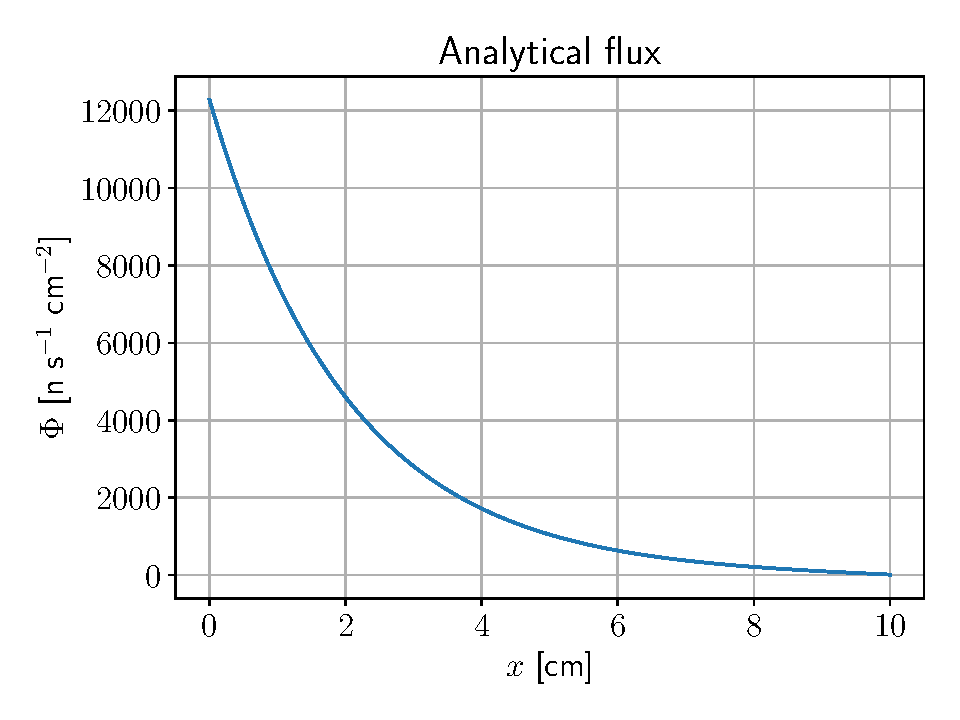
\includegraphics[width=10cm]{fig/Ex1_Analytical.pdf}
\centering
\caption{Analytical Solution for the neutron flux as a function of depth.}
\end{figure}
Flux values at the following locations (4 significant digits):\\
Flux value at $x_0$: 13.5896 n cm$^{-2}$ s$^{-1}$ \\
Flux value at $0$: 12276.8979 n cm$^{-2}$ s$^{-1}$ \\

\subsection{Question \#2}

Relationship between $\mathrm{\Phi}_i,\ \mathrm{\Phi}_{i+1},\ \mathrm{\Phi}_{i-1}$ at any point within the material:
\begin{equation}
    A \Phi_i + B \Phi_{i-1} +C \Phi_{i+1} = D
\end{equation}

Coefficients of the matrix A (4 significant digits), for a mesh size of 0.1cm:\\
Coef $A_{i,i}$: -16.6037 \\
Coef $A_{i-1,i}$: 8.2919 \\
Coef $A_{i+1,i}$: 8.2919 \\

Relationship between $\mathrm{\Phi}_i,\ \mathrm{\Phi}_{i-1},\ \mathrm{\Phi}_{i+1}$, \\
at the source:
\begin{equation}
    A \Phi_1 + B \Phi_{2} = C
\end{equation}
at the RHS of the problem:
\begin{equation}
    A \Phi_n + B \Phi_{n-1} = C
\end{equation}
Associated coefficients of the matrix A (4 significant digits), for a mesh size of 0.1cm:
at the source: \\
Coef $A_{1,i}$: -8.3119 \\
Coef $A_{2,i}$: 8.2919 \\
at the RHS: \\
Coef $A_{n-1,i}$: 8.2919 \\
Coef $A_{n,i}$: -12.1536 \\

\subsection{Question \#3}

Flux values from the numerical solver at the following locations (4 significant digits):\\
Flux value at $x_0$: 13.6244 \\
Flux value at $0$: 12280.5980 \\

Add two sentences describing what you see in Figure \ref{err} and a possible explanation :
The error decrease as the mech increase, meaning that the simulation converge. The order of convergence has been evaluated to $\sim  1$. 

\begin{figure}[H]
	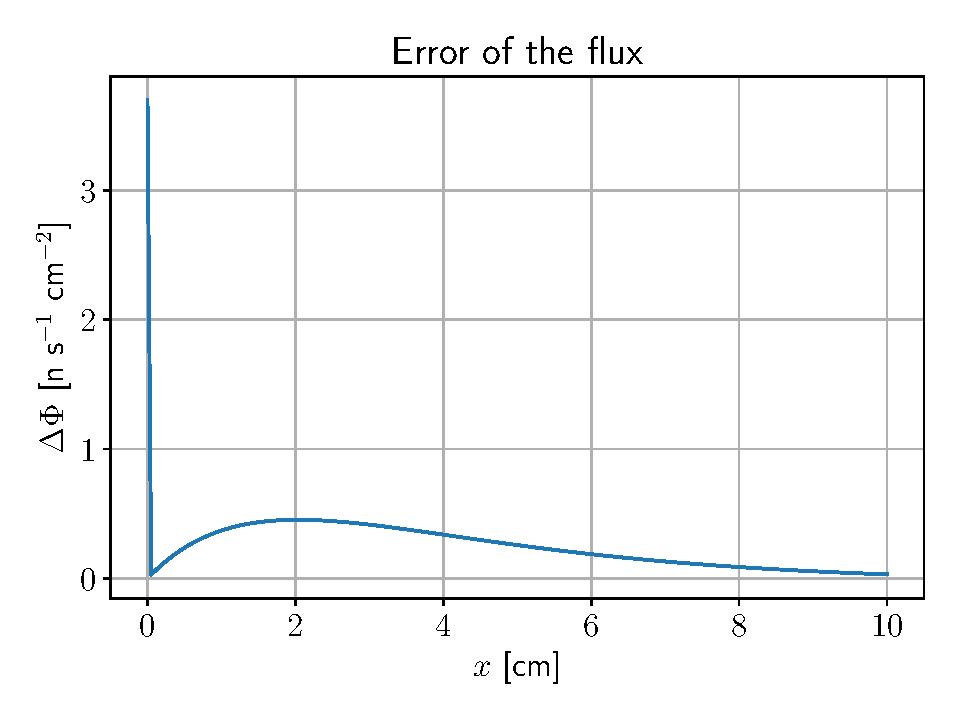
\includegraphics[width=10cm]{fig/Ex1_Error.pdf}
	\centering
	\caption{Distance between the solutions at each mesh point for a mesh size of 0.1 cm.}
\end{figure}

\begin{figure}[H]
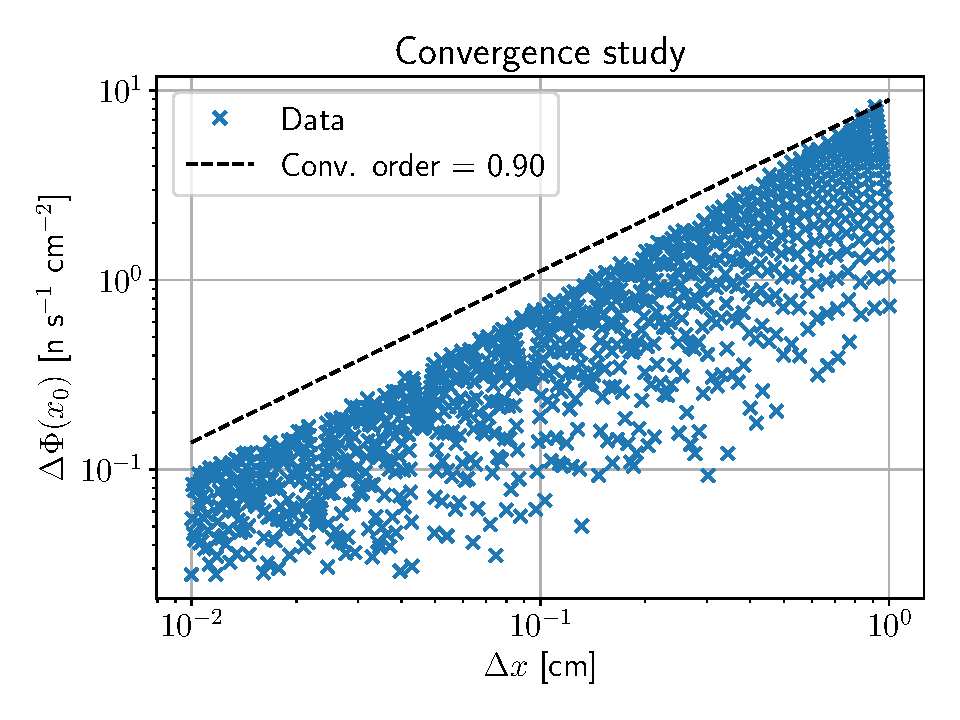
\includegraphics[width=10cm]{fig/Ex1_conv_N1000.pdf}
\centering
\caption{Evolution with mesh size of the absolute error of $\Phi(x_0)$.}
\label{err}
\end{figure}





% *******************************************************************************
% *** Exercice 2 ****************************************************************
% *******************************************************************************

\newpage
\section{Exercice \#2 - Modeling a planar reactor (1 group)}

\subsection{Question \#1}
\begin{figure}[H]
	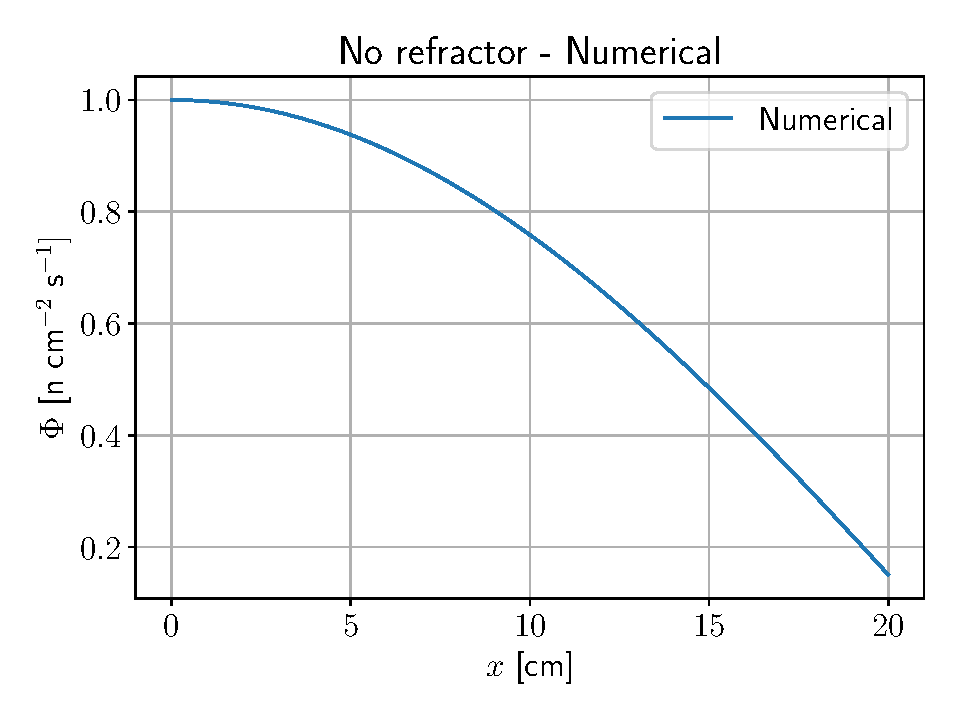
\includegraphics[width=10cm]{fig/Ex2_Q1.pdf}
	\centering
	\caption{Flux in the bare reactor for a mesh size of 0.1 cm.}
\end{figure}
Numerical solution for the bare system \\
keff (scientific format with 5 significant digits): 0.97305 \\
Net current at the core boundary (scientific format with 5 significant digits): 0.075436 \\

\subsection{Question \#2}
\begin{figure}[H]
	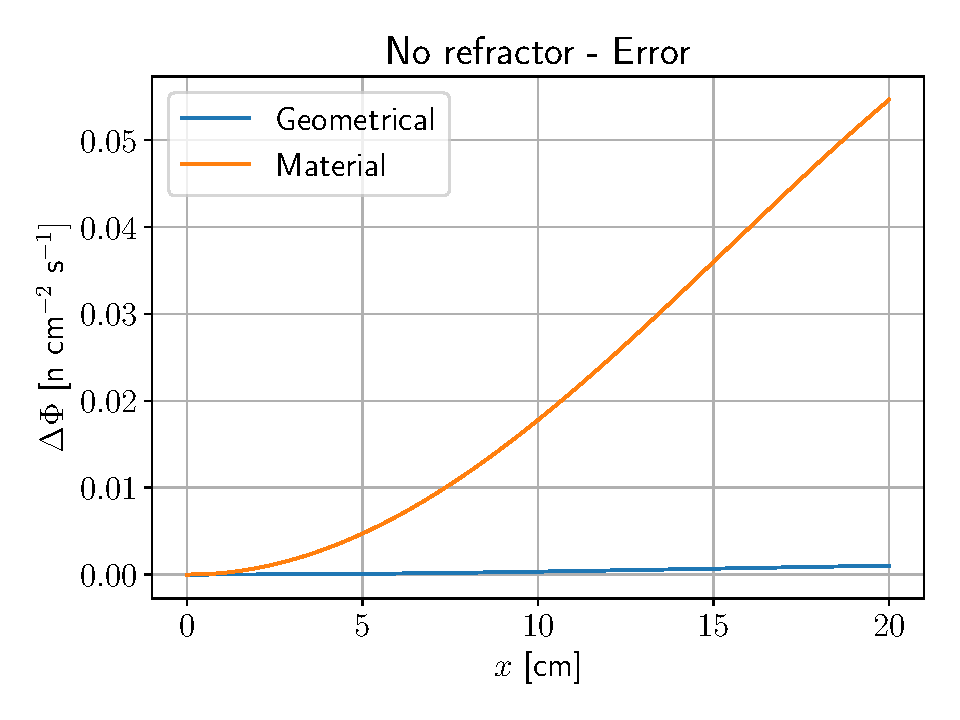
\includegraphics[width=10cm]{fig/Ex2_Q2.pdf}
	\centering
	\caption{Distance between the solutions at each mesh point for a mesh size of 0.1 cm.}
\end{figure}
Analytical solution for the bare system \\
keff (scientific format with 5 significant digits): 0.97356 \\
Net current at the core boundary (scientific format with 5 significant digits): 0.075367 \\

\subsection{Question \#3}
Numerical solution for the reflected system \\
keff (scientific format with 5 significant digits): 1.12038 \\
Net current at the core boundary (scientific format with 5 significant digits): -0.054402 \\
\begin{figure}[H]
	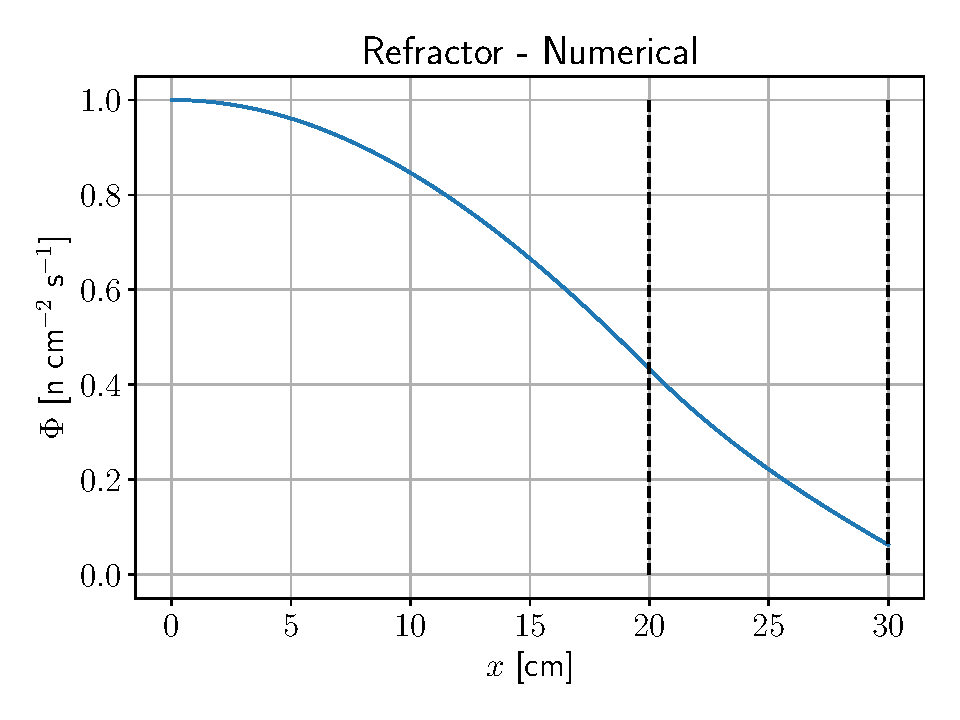
\includegraphics[width=10cm]{fig/Ex2_Q3.pdf}
	\centering
	\caption{Flux in the reflected reactor for a mesh size of 0.1 cm.}
\end{figure}





% *******************************************************************************
% *** Exercice 3 ****************************************************************
% *******************************************************************************

\newpage
\section{Exercice \#3 - Modeling a planar reactor (2 groups)}

\end{document}
